\section{実験装置}

\subsection{作用力測定装置}
本研究において使用した実験装置の概略図および写真を以下のFig,,Fig.に示す.

\subsection{校正実験装置}
本研究において製作・使用した実験装置の概略図および写真を以下のFig.,Fig.に示す.
校正装置は,作用力測定装置に取り付けられた2組のひずみセンサについて,
作用力の角度による出力電圧の関係性を調べる目的がある.
また,人為的な操作を可能な限り減らし自動化することで,
不本意なノイズの削減や実験回数を多くすることを実現することができた.
主に,自動一軸ステージ,自動回転ステージ,ロードセル,それらを接続するジョイントから構成される.
また,作用力測定装置と構成実験装置を固定するため,フレームを製作し作用力測定装置を取り付ける.
校正実験装置はアルミ板を介してフレームに取り付けることができるようになっている.
作用力測定装置をフレーム上に設置し,作用力測定装置の回転軸と自動回転ステージの回転軸を
できるだけ一致させるように調整をしながら設置する.

% \begin{figure}[htbp]
%     \footnotesize
%     \begin{center}
%         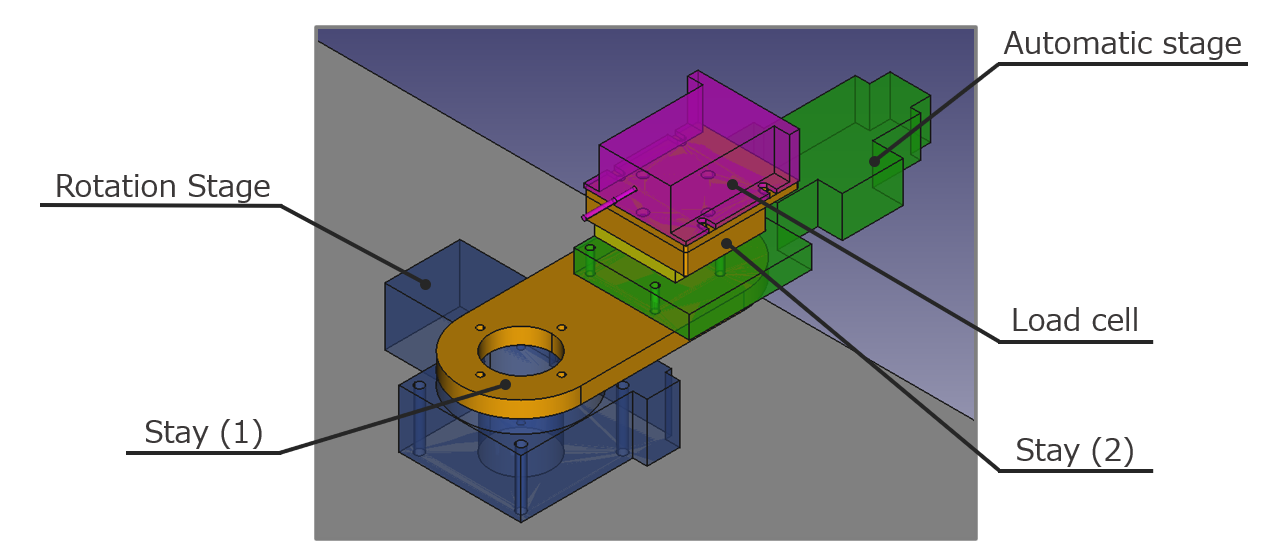
\includegraphics[width=95mm]{../images/21-1.png}
%         \caption{}
%     \end{center}
% \end{figure}

\subsection{測定理論}

\subsection{抗力・揚力における出力電圧勾配の理論式}

\begin{align}
    v_{x\; Theory} &= A \sin \left(\omega + \frac{3}{2} \pi\right) = A \cos \left(\omega + \pi\right) \\ 
    v_{y\; Theory} &= A \sin \left(\omega + \pi\right) = A \cos \left(\omega + \frac{1}{2} \pi\right) 
\end{align}
